% Supplemental material (separate PDF). Compile after main.tex so xr can read main.aux.
\documentclass[letterpaper,journal]{IEEEtran}
%\usepackage{ctex}
\usepackage{amsmath,amsfonts}
\usepackage{amsthm}
\usepackage{algorithmic}
\usepackage{algorithm}
\usepackage{array}
\usepackage[caption=false,font=normalsize,labelfont=sf,textfont=sf]{subfig}
\usepackage{textcomp}
\usepackage{stfloats}
\usepackage{url}
\usepackage{verbatim}
\usepackage{graphicx}
\usepackage{epsfig}
% \usepackage{subfigure}
\usepackage{epstopdf}
\usepackage{cite}
\usepackage{booktabs}
\usepackage{multirow} 
\usepackage{amssymb} 
\newtheorem{definition}{Definition}  
\newtheorem{theorem}{Theorem}
\newtheorem{proposition}{Proposition}
\newtheorem*{proposition*}{Proposition}

\newtheorem{assumption}{Assumption}
\newtheorem{lemma}{Lemma}
\newtheorem{corollary}{Corollary}
\newtheorem{remark}{Remark}
%\usepackage{appendix}
\usepackage{color}
\usepackage{placeins}
\def\red{\textcolor{red}}
\def\blue{\textcolor{black}}
\graphicspath{{./figures/}{./images/}}
\hyphenation{op-tical net-works semi-conduc-tor IEEE-Xplore}

\makeatletter
\newcommand{\rmnum}[1]{\romannumeral #1}
\newcommand{\Rmnum}[1]{\expandafter\@slowromancap\romannumeral #1@}
\makeatother

\renewcommand{\topfraction}{0.99}
\renewcommand{\bottomfraction}{0.99}
\renewcommand{\textfraction}{0.01}
\renewcommand{\floatpagefraction}{0.99}
\renewcommand{\dbltopfraction}{0.9}
\renewcommand{\dblfloatpagefraction}{0.9}
\setlength{\dbltextfloatsep}{8pt plus 2pt}
\setcounter{topnumber}{5}
\setcounter{bottomnumber}{5}
\setcounter{totalnumber}{10}


\usepackage{xr}
\externaldocument{main}

\begin{document}

\title{Supplemental Material for\\
RAVEN-MCS: Target-Risk-Calibrated Windowed-Asynchronous Federated Data Completion for Mobile Crowdsensing under Two-Stage Non-Random Selection}

\author{**** and Anfeng Liu}

\maketitle

\noindent\textit{This file is supplemental material for the companion main paper
and must be uploaded as a separate PDF. It is not a standalone submission.}

% Continue figure/table/equation numbers from the companion main paper.
% Update the three counters if the main-paper last numbers change.
\setcounter{figure}{5}
\setcounter{table}{5}
\setcounter{equation}{50}

\appendices
\section{Complete Proofs for Sections III--VI}
\label{app:complete_proofs}

This appendix provides the complete proofs deferred from
Section~\ref{sec:theory}.  All notation and assumptions are inherited from
Sections~\ref{sec:system_model}--\ref{sec:theory}.  In particular,
$\boldsymbol\varpi^{\mathrm{tar}}$ is the public atomic deployment-target law,
and $\pi^{\mathrm{tar}}_{k,i}$ is the compatible client--atomic target law.
$P_r^{\mathrm{opp}}(k,i)$ is the opportunity-event law, while
$p^{\mathrm{obs}}_{k,r,i}$ and $q^{\mathrm{use}}_{k,r}$ are sequential
pre-outcome selection probabilities.  Finally, $\mathcal{C}_r$ is the feasible
aggregation set of (P2).

\subsection{Proof of Proposition~1}
\label{app:proof_prop1}

\begin{proposition*}[Target-vs-arrival risk distinction]
Let $\boldsymbol\varpi^{\mathrm{tar}}$ and
$\widetilde{\boldsymbol\rho}^{\mathrm{arr}}$ be two normalized laws on the same
finite supported atomic domain.  If
$\boldsymbol\varpi^{\mathrm{tar}}\neq
\widetilde{\boldsymbol\rho}^{\mathrm{arr}}$, then there exists a bounded
nonnegative error profile $e_i$ such that
\begin{equation}
    \sum_i \varpi_i^{\mathrm{tar}}e_i
    \neq
    \sum_i \widetilde\rho_i^{\mathrm{arr}}e_i.
    \label{eq:app_prop1_claim}
\end{equation}
Conversely, equality of the two weighted expectations for every bounded error
profile implies equality of the two underlying laws.
\end{proposition*}

\noindent\emph{Proof.}
Define $d_i\triangleq\varpi_i^{\mathrm{tar}}-\widetilde\rho_i^{\mathrm{arr}}$.
Because both vectors are probability laws,
\begin{equation}
    \sum_i d_i=0.
    \label{eq:app_prop1_zero_sum}
\end{equation}
The assumption
$\boldsymbol\varpi^{\mathrm{tar}}\neq
\widetilde{\boldsymbol\rho}^{\mathrm{arr}}$
implies that $d_i\neq0$ for at least one atomic unit.  Hence the set
$B_+\triangleq\{i:d_i>0\}$
is nonempty.  Indeed, if $d_i\le0$ for every $i$, then
\eqref{eq:app_prop1_zero_sum} would force $d_i=0$ for every $i$, contradicting
the assumed inequality of the two laws.

Choose the bounded nonnegative profile
$e_i=\mathbf{1}\{i\in B_+\}$.
Then
\begin{align}
 &
 \sum_i
 \varpi_i^{\mathrm{tar}}e_i
 -
 \sum_i
 \widetilde\rho_i^{\mathrm{arr}}e_i
 \nonumber\\
 &\qquad=
 \sum_{i\in B_+}
 \left(
 \varpi_i^{\mathrm{tar}}
 -
 \widetilde\rho_i^{\mathrm{arr}}
 \right)
 =
 \sum_{i\in B_+}d_i
 >0.
 \label{eq:app_prop1_difference}
\end{align}
Therefore, the two weighted expectations differ for the bounded nonnegative
profile $e_i=\mathbf{1}\{i\in B_+\}$.  This proves the forward direction.

For the converse, suppose
\begin{equation}
    \sum_i \varpi_i^{\mathrm{tar}}e_i
    =
    \sum_i \widetilde\rho_i^{\mathrm{arr}}e_i
    \label{eq:app_prop1_all_equal}
\end{equation}
for every bounded error profile $e$.  Fix an arbitrary atomic unit $j$ and set
$e_i^{(j)}=\mathbf{1}\{i=j\}$.
Substituting $e_i^{(j)}$ into
\eqref{eq:app_prop1_all_equal} gives
$\varpi_j^{\mathrm{tar}}=\widetilde\rho_j^{\mathrm{arr}}$.
Since $j$ was arbitrary, the equality holds for every coordinate.  Hence
$\boldsymbol\varpi^{\mathrm{tar}}=\widetilde{\boldsymbol\rho}^{\mathrm{arr}}$.
This proves the converse. \hfill$\square$

\paragraph{Interpretation.}
The proposition proves that the two probability laws induce different linear
risk functionals whenever the laws differ.  It does not claim that a particular
fixed predictor must exhibit a nonzero numerical gap.  Nor does it claim that
the minimizers must differ for every restricted model class.


\subsection{Proof of Proposition~2}
\label{app:proof_prop2}

\begin{proposition*}[Normalized target reconstruction]
Under A1--A3, for any bounded function $\phi(k,i)$, the H\'ajek ratio in
\eqref{eq:hajek_phi} converges in probability to
\begin{equation}
    \Phi^{\mathrm{tar}}
    =
    \sum_{k,i}
    \pi^{\mathrm{tar}}_{k,i}\phi(k,i).
    \label{eq:app_target_phi}
\end{equation}
\end{proposition*}

\noindent\emph{Proof.}
We first record two identities used by the proof.

\subsubsection{Target-Measure Compatibility}

For every stratum $s$ with $\Lambda_s^{\mathrm{tar}}>0$,
\eqref{eq:target_conditional_atomic} gives
\begin{equation}
    \sum_{i:s(i)=s}
    \nu^{\mathrm{tar}}_{i\mid s}
    =
    \frac{
    \sum_{i:s(i)=s}\varpi_i^{\mathrm{tar}}
    }{
    \Lambda_s^{\mathrm{tar}}
    }
    =1.
    \label{eq:app_nu_normalization}
\end{equation}
For an atomic unit $i$ whose stratum has positive target mass, using
$\pi^{\mathrm{tar}}_{k,s}
=\Lambda_s^{\mathrm{tar}}
\lambda^{\mathrm{tar}}_{k\mid s}$ and
$\sum_k\lambda^{\mathrm{tar}}_{k\mid s}=1$ gives
\begin{align}
 \sum_k\pi^{\mathrm{tar}}_{k,i}
 &=
 \sum_k
 \pi^{\mathrm{tar}}_{k,s(i)}
 \nu^{\mathrm{tar}}_{i\mid s(i)}
 \nonumber\\
 &=
 \Lambda_{s(i)}^{\mathrm{tar}}
 \nu^{\mathrm{tar}}_{i\mid s(i)}
 \sum_k
 \lambda^{\mathrm{tar}}_{k\mid s(i)}
 \nonumber\\
 &=
 \Lambda_{s(i)}^{\mathrm{tar}}
 \frac{\varpi_i^{\mathrm{tar}}}
 {\Lambda_{s(i)}^{\mathrm{tar}}}
 =
 \varpi_i^{\mathrm{tar}}.
 \label{eq:app_target_compatibility_positive}
\end{align}
If instead $\Lambda_{s(i)}^{\mathrm{tar}}=0$, then nonnegativity and
\eqref{eq:target_stratum_mass} imply $\varpi_i^{\mathrm{tar}}=0$.  The
zero-stratum convention in
\eqref{eq:target_ks_mass}--\eqref{eq:target_ki_mass}
gives $\pi^{\mathrm{tar}}_{k,i}=0$ for every $k$.  Hence, in both cases,
\begin{equation}
 \sum_k\pi^{\mathrm{tar}}_{k,i}
 =\varpi_i^{\mathrm{tar}}.
 \label{eq:app_target_compatibility}
\end{equation}
Summing over $i$ also yields
\begin{equation}
    \sum_{k,i}\pi^{\mathrm{tar}}_{k,i}
    =
    \sum_i\varpi_i^{\mathrm{tar}}
    =1.
    \label{eq:app_pi_normalized}
\end{equation}

\subsubsection{Sequential Inverse-Selection Identity}

Consider an opportunity event $e\in\mathcal{O}_r$ with mark
$(k_e,i_e)=(k,i)$.  For compactness, write
$p_e\triangleq p^{\mathrm{obs}}_{k,r,i}$ and
$q_{k,r}\triangleq q^{\mathrm{use}}_{k,r}$.
Under A1, both denominators are strictly positive on the target-supported event.

Let $\mathcal{H}^{\mathrm{obs}}_e$ denote the legal history immediately before
the observation outcome.  By the definition of $p_e$ and A2,
\begin{equation}
    \mathbb{E}
    \left[
    \left.
    \frac{O_e}{p_e}
    \right|
    k_e=k,\,
    i_e=i,\,
    \mathcal{H}^{\mathrm{obs}}_e
    \right]
    =1.
    \label{eq:app_obs_ipw}
\end{equation}
If $O_e=1$, client $k$ has at least one observed item and is therefore in the
registered-attempt set $\mathcal{E}_r$.  Conditional on the legal pre-$U$
history $\mathcal{H}^{\mathrm{use}}_{k,r}$, the definition of $q_{k,r}$ and A2
give
\begin{equation}
    \mathbb{E}
    \left[
    \left.
    \frac{U_{k,r}}{q_{k,r}}
    \right|
    k\in\mathcal{E}_r,\,
    \mathcal{H}^{\mathrm{use}}_{k,r}
    \right]
    =1.
    \label{eq:app_use_ipw}
\end{equation}
The usable-update indicator may be shared by several observed opportunity
events of the same client-window.  This induces within-window dependence, but
it does not invalidate the conditional identity
\eqref{eq:app_use_ipw}.  A3 handles such dependence at the
cluster/window level.

Applying the tower property in the temporal order
opportunity $\rightarrow$ observation $\rightarrow$ registration/use, and using
\eqref{eq:A2_use_mean_ignorability} on the $O_e=1$ branch, gives
\begin{align}
 &\mathbb{E}\!\left[
 \left.
 \frac{O_eU_{k,r}}{p_eq_{k,r}}
 \right|
 k_e=k,\,i_e=i,\,\mathcal{H}^{\mathrm{obs}}_e
 \right]
 \nonumber\\
 &\qquad=
 \mathbb{E}\!\left[
 \left.
 \frac{O_e}{p_e}
 \right|
 k_e=k,\,i_e=i,\,\mathcal{H}^{\mathrm{obs}}_e
 \right]
 =1.
 \label{eq:app_sequential_identity}
\end{align}
The inner conditional expectation is evaluated only on the $O_e=1$ branch,
where client $k$ is registered.  It equals one by the strengthened
mean-ignorability condition \eqref{eq:A2_use_mean_ignorability}.  The outer
expectation is then \eqref{eq:app_obs_ipw}.

With these two identities in hand, we prove the proposition.
For event $e\in\mathcal{O}_r$, recall
\begin{equation}
 \chi_e
 =
 O_eU_{k_e,r}
 \frac{
 \pi^{\mathrm{tar}}_{k_e,i_e}
 }{
 P_r^{\mathrm{opp}}(k_e,i_e)
 p^{\mathrm{obs}}_{k_e,r,i_e}
 q^{\mathrm{use}}_{k_e,r}
 }.
 \label{eq:app_chi}
\end{equation}
Condition first on the opportunity mark $(k_e,i_e)=(k,i)$.  Using
\eqref{eq:app_sequential_identity},
\begin{align}
 &\mathbb{E}
 \left[
 \left.
 \chi_e\phi(k_e,i_e)
 \right|
 k_e=k,\,
 i_e=i
 \right]
 \nonumber\\
 &=
 \frac{
 \pi^{\mathrm{tar}}_{k,i}
 }{
 P_r^{\mathrm{opp}}(k,i)
 }
 \phi(k,i)
 \,
 \mathbb{E}
 \left[
 \left.
 \frac{
 O_eU_{k,r}
 }{
 p^{\mathrm{obs}}_{k,r,i}
 q^{\mathrm{use}}_{k,r}
 }
 \right|
 k_e=k,\,
 i_e=i
 \right]
 \nonumber\\
 &=
 \frac{
 \pi^{\mathrm{tar}}_{k,i}
 }{
 P_r^{\mathrm{opp}}(k,i)
 }
 \phi(k,i).
 \label{eq:app_conditional_weighted_moment}
\end{align}
By \eqref{eq:opp_event_law}, the mark itself has opportunity law
$P_r^{\mathrm{opp}}(k,i)$.  Averaging
\eqref{eq:app_conditional_weighted_moment} over this law therefore yields
\begin{align}
 \mathbb{E}
 \left[
 \chi_e\phi(k_e,i_e)
 \right]
 &=
 \sum_{k,i}
 P_r^{\mathrm{opp}}(k,i)
 \frac{
 \pi^{\mathrm{tar}}_{k,i}
 }{
 P_r^{\mathrm{opp}}(k,i)
 }
 \phi(k,i)
 \nonumber\\
 &=
 \sum_{k,i}
 \pi^{\mathrm{tar}}_{k,i}\phi(k,i)
 =
 \Phi^{\mathrm{tar}}.
 \label{eq:app_expected_numerator_event}
\end{align}
Likewise, taking $\phi\equiv1$ and using
\eqref{eq:app_pi_normalized},
\begin{equation}
    \mathbb{E}[\chi_e]
    =
    \sum_{k,i}\pi^{\mathrm{tar}}_{k,i}
    =1.
    \label{eq:app_expected_denominator_event}
\end{equation}

Let
\begin{equation}
    N_R^{\mathrm{opp}}
    \triangleq
    \sum_{r=0}^{R-1}|\mathcal{O}_r|
    \label{eq:app_total_opp_events}
\end{equation}
be the total number of opportunity events in the first $R$ windows.  Define
\begin{align}
 A_R(\phi)
 &\triangleq
 \sum_{r<R}
 \sum_{e\in\mathcal{O}_r}
 \chi_e\phi(k_e,i_e),
 \label{eq:app_AR}\\
 B_R
 &\triangleq
 \sum_{r<R}
 \sum_{e\in\mathcal{O}_r}
 \chi_e.
 \label{eq:app_BR}
\end{align}
A3 explicitly requires the asymptotic regime
$N_R^{\mathrm{opp}}\rightarrow\infty$.  It is precisely the regularity
condition needed to pass from the eventwise identities above to the possibly
dependent client-window process.  Along this growing sequence, it gives
\begin{align}
 \frac{A_R(\phi)}{N_R^{\mathrm{opp}}}
 &\xrightarrow{p}
 \Phi^{\mathrm{tar}},
 \label{eq:app_AR_lln}\\
 \frac{B_R}{N_R^{\mathrm{opp}}}
 &\xrightarrow{p}
 1.
 \label{eq:app_BR_lln}
\end{align}
The second limit is strictly positive.  Therefore, by the continuous mapping
theorem (equivalently, Slutsky's theorem),
\begin{align}
 \widehat\Phi_R
 &=
 \frac{A_R(\phi)}{B_R}
 =
 \frac{
 A_R(\phi)/N_R^{\mathrm{opp}}
 }{
 B_R/N_R^{\mathrm{opp}}
 }
 \xrightarrow{p}
 \Phi^{\mathrm{tar}}.
 \label{eq:app_hajek_limit}
\end{align}
This proves the main convergence statement.

It remains to verify the two stated marginals.

First, fix $(k_0,s_0)$ and choose
\begin{equation}
    \phi_{k_0,s_0}(k,i)
    =
    \mathbf{1}\{k=k_0,\ s(i)=s_0\}.
    \label{eq:app_phi_client_stratum}
\end{equation}
If $\Lambda_{s_0}^{\mathrm{tar}}>0$, then
\begin{align}
 \Phi^{\mathrm{tar}}
 &=
 \sum_{i:s(i)=s_0}
 \pi^{\mathrm{tar}}_{k_0,i}
 \nonumber\\
 &=
 \pi^{\mathrm{tar}}_{k_0,s_0}
 \sum_{i:s(i)=s_0}
 \nu^{\mathrm{tar}}_{i\mid s_0}
 =
 \pi^{\mathrm{tar}}_{k_0,s_0},
 \label{eq:app_recover_client_stratum_positive}
\end{align}
where the last equality follows from
\eqref{eq:app_nu_normalization}.  If
$\Lambda_{s_0}^{\mathrm{tar}}=0$, the zero-stratum convention gives both
$\pi^{\mathrm{tar}}_{k_0,s_0}=0$ and
$\pi^{\mathrm{tar}}_{k_0,i}=0$ for every $i$ in that stratum.  The same
conclusion then holds.  Thus, in all cases,
$\Phi^{\mathrm{tar}}=\pi^{\mathrm{tar}}_{k_0,s_0}$.

Second, fix a deployment group $g$ and choose
$\phi_g(k,i)=\mathbf{1}\{h(i)=g\}$.
Using target compatibility
\eqref{eq:app_target_compatibility},
\begin{align}
 \Phi^{\mathrm{tar}}
 &=
 \sum_{k,i}
 \pi^{\mathrm{tar}}_{k,i}
 \mathbf{1}\{h(i)=g\}
 \nonumber\\
 &=
 \sum_{i:h(i)=g}
 \sum_k
 \pi^{\mathrm{tar}}_{k,i}
 \nonumber\\
 &=
 \sum_{i:h(i)=g}
 \varpi_i^{\mathrm{tar}}
 =
 \mu_g.
 \label{eq:app_recover_group}
\end{align}
Hence, the ideal normalized sequential correction recovers both the
client--stratum target law and, through the compatibility bridge, the
deployment-group target law. \hfill$\square$

\paragraph{Scope of Proposition~2.}
The result is an identification/consistency statement for the ideal pooled
sequential ratios.  It does not imply that every finite-window normalized
reference $\boldsymbol\beta_r^\star$ exactly realizes the deployment target.
The current mobile support can make exact realization infeasible, even when
the pooled sequential weights have the correct target-law interpretation.  This
is the role of the feasibility-aware calibration in
Section~\ref{sec:calibration}.  The result also does not assert exact
unbiasedness of the finite-sample clipped plug-in implementation.  When the
stabilization bounds are active, the practical estimator deliberately trades
exact inverse-weight identification for controlled weight concentration.


\subsection{Proof of Theorem~1}
\label{app:proof_theorem1}

\noindent\textbf{Theorem~1.}
Under A4, every active window has a nonempty compact convex feasible set
$\mathcal{C}_r$, and the calibration program
$\min_{\boldsymbol\alpha\in\mathcal{C}_r}J_r(\boldsymbol\alpha)$
has a unique global minimizer $\boldsymbol\alpha_r^\star$.

\noindent\emph{Proof.}
Fix an active window $r$.  Then
\begin{equation}
    K_r=|\mathcal{A}_r|\ge1.
    \label{eq:app_K_positive}
\end{equation}
Consider the uniform vector
\begin{equation}
    \boldsymbol\alpha_r^{u}
    =
    \frac{1}{K_r}\mathbf{1}.
    \label{eq:app_uniform_alpha}
\end{equation}
It satisfies
\begin{equation}
    \mathbf{1}^{\top}\boldsymbol\alpha_r^{u}=1
    \quad\text{and}\quad
    \alpha_{k,r}^{u}=\frac{1}{K_r}\ge0.
    \label{eq:app_uniform_simplex}
\end{equation}
From \eqref{eq:cap_ess},
\begin{equation}
    \overline\alpha_r
    =
    \min\left\{
    1,
    \max\left\{
    \alpha_{\max},
    \frac{1}{K_r}
    \right\}
    \right\}.
    \label{eq:app_alpha_bar}
\end{equation}
Since $K_r\ge1$ and $0<\alpha_{\max}\le1$,
\begin{equation}
    \frac{1}{K_r}\le\overline\alpha_r\le1.
    \label{eq:app_uniform_box}
\end{equation}
Thus the box constraints are satisfied by
$\boldsymbol\alpha_r^{u}$.

Next,
\begin{equation}
    \left\|
    \boldsymbol\alpha_r^{u}
    \right\|_2^2
    =
    K_r\left(\frac{1}{K_r}\right)^2
    =
    \frac{1}{K_r}.
    \label{eq:app_uniform_l2}
\end{equation}
Because
\begin{equation}
    \overline E_r
    =
    \min\{E_{\min},K_r\}
    \le K_r,
    \label{eq:app_Ebar_leq_K}
\end{equation}
we have
\begin{equation}
    \frac{1}{K_r}
    \le
    \frac{1}{\overline E_r}.
    \label{eq:app_uniform_ess}
\end{equation}
Therefore
\begin{equation}
    \boldsymbol\alpha_r^{u}
    \in
    \mathcal{C}_r,
    \label{eq:app_C_nonempty}
\end{equation}
so $\mathcal{C}_r$ is nonempty.

The equality constraint
$\mathbf{1}^{\top}\boldsymbol\alpha=1$ defines an affine set.  The coordinate
constraints
$0\le\alpha_k\le\overline\alpha_r$ define a closed convex box, and
\begin{equation}
    \left\{
    \boldsymbol\alpha:
    \|\boldsymbol\alpha\|_2^2
    \le
    1/\overline E_r
    \right\}
    \label{eq:app_l2_ball}
\end{equation}
is a closed convex Euclidean ball.  Their intersection is therefore closed and
convex.  Moreover, the simplex and box constraints imply
$0\le\alpha_k\le1$ for every coordinate, so the set is bounded.  Hence
$\mathcal{C}_r$ is compact.

We now analyze the objective.  Expanding only the terms that are quadratic in
$\boldsymbol\alpha$, the Hessian of $J_r$ is
\begin{equation}
 \nabla^2J_r
 =
 \lambda_gM_r^{\top}M_r
 +
 \lambda_{\beta}I
 +
 \lambda_vV_r.
 \label{eq:app_P2_hessian}
\end{equation}
The debt term
$-\mathbf{Q}_r^{\top}M_r\boldsymbol\alpha$ and the staleness term
$\lambda_s\overline{\boldsymbol\tau}_r^{\top}\boldsymbol\alpha$ are linear.
They therefore contribute zero Hessian.  Under A4,
\begin{equation}
    M_r^{\top}M_r\succeq0,
    \qquad
    V_r\succeq0,
    \qquad
    \lambda_g,\lambda_v\ge0,
    \qquad
    \lambda_{\beta}>0.
    \label{eq:app_psd_terms}
\end{equation}
Consequently, for every nonzero vector $\mathbf{x}\in\mathbb{R}^{K_r}$,
\begin{align}
 \mathbf{x}^{\top}\nabla^2J_r\mathbf{x}
 &=
 \lambda_g\|M_r\mathbf{x}\|_2^2
 +
 \lambda_{\beta}\|\mathbf{x}\|_2^2
 +
 \lambda_v\mathbf{x}^{\top}V_r\mathbf{x}
 \nonumber\\
 &\ge
 \lambda_{\beta}\|\mathbf{x}\|_2^2
 >0.
 \label{eq:app_strong_convex}
\end{align}
Thus $J_r$ is $\lambda_{\beta}$-strongly convex on
$\mathbb{R}^{K_r}$ and hence strictly convex on $\mathcal{C}_r$.

Because $J_r$ is continuous and $\mathcal{C}_r$ is nonempty and compact, the
Weierstrass theorem guarantees the existence of at least one minimizer.
Strict convexity on the convex feasible set guarantees that two distinct
minimizers cannot exist.  Therefore, (P2) has exactly one global minimizer,
denoted by $\boldsymbol\alpha_r^\star$.  This completes the proof.
\hfill$\square$

\paragraph{Scope of Theorem~1.}
The theorem proves existence and uniqueness of the mathematical optimizer of
(P2).  It does not, by itself, certify that a finite-precision solver log
reconstructs that optimizer exactly.  Numerical feasibility and post-hoc
solver audit are separate empirical/provenance questions.


\subsection{Proof of Proposition~3}
\label{app:proof_prop3}

\noindent\textbf{Proposition~3.}
Assume A1, A4, and A5.  Then the implemented clipped plug-in
$\widehat{\boldsymbol\beta}_r$ is a Lipschitz perturbation of the
same-window ideal reference $\boldsymbol\beta_r^\star$, and the P2 map
does not amplify that $\ell_2$ error on a fixed feasible set.

\noindent\emph{Proof.}
Fix an active window $r$ and the common set $\mathcal{A}_r$.
Write $\widetilde a_{k,r,i}=\widehat\zeta^{o}_{k,r,i}/
\max\{\widehat p^{\mathrm{obs}}_{k,r,i},p_{\min}\}$ and
$\widetilde d_{k,r}=1/\max\{\widehat q^{\mathrm{use}}_{k,r},q_{\min}\}$,
so that
$a=\widetilde a-(\widetilde a-a_{\max})_+$ and
$d=\widetilde d-(\widetilde d-d_{\max})_+$.
The clipping residuals are collected in
$\varepsilon_{\mathrm{clip}}$; they are not set to zero.

On target support, $\zeta=\pi^{\mathrm{tar}}/\pi^{\mathrm{opp}}$ and
$\widehat\zeta=\pi^{\mathrm{tar}}/\max\{\widehat\pi^{\mathrm{opp}},
\pi_{\min}\}$.  A5 and $\pi^{\mathrm{tar}}\le1$ give
$\lvert\widehat\zeta-\zeta\rvert\le\varepsilon_\pi/\pi_{\min}^2$ and
\begin{equation}
 \bigl\lvert\widetilde a-a^\star\bigr\rvert
 \le
 \frac{\varepsilon_\pi}{\pi_{\min}^2 p_{\min}}
 +\frac{\varepsilon_p}{\pi_{\min}\,p_{\min}\,p_{\min}^{\mathrm{true}}},
 \qquad
 \bigl\lvert\widetilde d-d^\star\bigr\rvert
 \le
 \frac{\varepsilon_q}{q_{\min}q_{\min}^{\mathrm{true}}}.
 \label{eq:app_plugin_lipschitz}
\end{equation}
With $n_r=\max_{k\in\mathcal{A}_r}\sum_i R_{k,r,i}O_{k,r,i}$,
$m_k\le n_r a_{\max}$, and
$d^\star\le 1/q_{\min}^{\mathrm{true}}\le d_{\max}$,
the unnormalized masses satisfy
\begin{equation}
 \|b-b^\star\|_1
 \le
 K_r n_r
 \Bigl(
 \tfrac{d_{\max}}{\pi_{\min}^2 p_{\min}}\varepsilon_\pi
 +\tfrac{d_{\max}}{\pi_{\min}p_{\min}p_{\min}^{\mathrm{true}}}\varepsilon_p
 +\tfrac{a_{\max}}{q_{\min}q_{\min}^{\mathrm{true}}}\varepsilon_q
 +(a_{\max}+d_{\max})\varepsilon_{\mathrm{clip}}
 \Bigr).
 \label{eq:app_plugin_mass}
\end{equation}
The H\'ajek map $b\mapsto b/(\mathbf{1}^{\top}b)$ is
$2/B_{\min}$-Lipschitz in $\ell_1$ on
$\{b\ge0:\mathbf{1}^{\top}b\ge B_{\min}\}$, which yields
\eqref{eq:g4_beta} with the displayed $C_1$.
The P2 bound \eqref{eq:g4_alpha} is the already-proved reference
non-expansion \eqref{eq:app_reference_nonexpansive} on the common
convex set $\mathcal{C}_r$.  The composition bound
\eqref{eq:g4_comp} is the operator $2$-norm.
\hfill$\square$

The constant $C_1$ is a worst-case envelope.  It is not a numerical
RMSE certificate, and the argument does not apply when Design changes
$\mathcal{A}_r$.


\subsection{Proof of the Target-Debt Accounting Bound}
\label{app:proof_debt_bound}

The bound states that the prefix-averaged deployment composition
$\overline{\boldsymbol\omega}_R$ cannot drift farther from the target
$\boldsymbol\mu$ than twice the accumulated target debt per unit of active
step mass.  Intuitively, the debt vector records, for each deployment group,
how much service the group has cumulatively missed across windows.  The
relation therefore turns that accounting into a deterministic control on
structural mismatch: the group-average distance to the target is bounded by
how much the process has fallen behind, normalized by how much it has run.
The proof proceeds in three steps.  It first shows that the coordinate-wise
debt dominates the cumulative signed discrepancy.  It then combines this
domination with the zero-sum property of the discrepancy to bound its
$\ell_1$ norm by twice the debt.  Finally, it divides by the active step
mass $S_R$ to obtain the stated bound.

We now prove the deterministic relation in
\eqref{eq:debt_bound}.  Recall
\begin{equation}
    S_R
    =
    \sum_{r=0}^{R-1}\eta_rI_r,
    \qquad
    \overline{\boldsymbol\omega}_R
    =
    \frac{
    \sum_{r=0}^{R-1}
    \eta_rI_r\boldsymbol\omega_r
    }{S_R},
    \label{eq:app_debt_prefix_defs}
\end{equation}
for $S_R>0$.  In every active window,
$\boldsymbol\alpha_r$ is a probability vector and each column
$\mathbf{c}_{k,r}^{g}$ of $M_r$ is a deployment-group probability vector.
Therefore
\begin{equation}
    \boldsymbol\omega_r
    =
    M_r\boldsymbol\alpha_r
    \in
    \Delta^{|\mathcal G|-1},
    \label{eq:app_omega_simplex}
\end{equation}
and hence
\begin{equation}
    \mathbf{1}^{\top}\boldsymbol\omega_r
    =
    \mathbf{1}^{\top}\boldsymbol\mu
    =1.
    \label{eq:app_equal_mass}
\end{equation}

Define the cumulative signed target discrepancy
\begin{equation}
    \mathbf{D}_R
    \triangleq
    \sum_{r=0}^{R-1}
    \eta_rI_r
    \left(
    \boldsymbol\mu-\boldsymbol\omega_r
    \right).
    \label{eq:app_DR}
\end{equation}
By \eqref{eq:app_debt_prefix_defs},
\begin{equation}
    \mathbf{D}_R
    =
    S_R
    \left(
    \boldsymbol\mu-\overline{\boldsymbol\omega}_R
    \right).
    \label{eq:app_DR_baromega}
\end{equation}

Fix a target-group coordinate $g$.  In an active window, the debt recursion is
\begin{equation}
    Q_{r+1,g}
    =
    \left[
    Q_{r,g}
    +
    \eta_r
    \left(
    \mu_g-\omega_{r,g}
    \right)
    \right]_+.
    \label{eq:app_debt_coordinate}
\end{equation}
Since $[x]_+\ge x$ for every scalar $x$,
\begin{equation}
    Q_{r+1,g}
    \ge
    Q_{r,g}
    +
    \eta_r
    \left(
    \mu_g-\omega_{r,g}
    \right)
    \label{eq:app_debt_one_step}
\end{equation}
holds for active windows.  In inactive windows,
$Q_{r+1,g}=Q_{r,g}$ and $I_r=0$.  The same inequality can therefore be written
uniformly as
\begin{equation}
    Q_{r+1,g}
    \ge
    Q_{r,g}
    +
    \eta_rI_r
    \left(
    \mu_g-\omega_{r,g}
    \right).
    \label{eq:app_debt_one_step_all}
\end{equation}
Telescoping from $r=0$ to $R-1$ and using $Q_{0,g}=0$ gives
\begin{equation}
    Q_{R,g}
    \ge
    D_{R,g}.
    \label{eq:app_Q_dominates_D}
\end{equation}
Because $Q_{R,g}\ge0$, it follows that
\begin{equation}
    (D_{R,g})_+
    \le
    Q_{R,g}.
    \label{eq:app_positive_part_domination}
\end{equation}
Summing over $g$,
\begin{equation}
    \|(\mathbf{D}_R)_+\|_1
    \le
    \|\mathbf{Q}_R\|_1.
    \label{eq:app_positive_part_l1}
\end{equation}

Next, by \eqref{eq:app_equal_mass},
\begin{align}
    \mathbf{1}^{\top}\mathbf{D}_R
    &=
    \sum_{r=0}^{R-1}
    \eta_rI_r
    \mathbf{1}^{\top}
    \left(
    \boldsymbol\mu-\boldsymbol\omega_r
    \right)
    \nonumber\\
    &=
    \sum_{r=0}^{R-1}
    \eta_rI_r(1-1)
    =0.
    \label{eq:app_DR_zero_sum}
\end{align}
For any finite-dimensional vector with zero coordinate sum, the positive and
negative parts have equal $\ell_1$ mass:
\begin{equation}
    \|(\mathbf{D}_R)_+\|_1
    =
    \|(\mathbf{D}_R)_-\|_1,
    \label{eq:app_pos_neg_equal}
\end{equation}
where $(\mathbf{x})_-=[-\mathbf{x}]_+$.  Therefore
\begin{equation}
\begin{aligned}
    \|\mathbf{D}_R\|_1
    &=
    \|(\mathbf{D}_R)_+\|_1
    +
    \|(\mathbf{D}_R)_-\|_1\\
    &=2\|(\mathbf{D}_R)_+\|_1
    \le
    2\|\mathbf{Q}_R\|_1.
\end{aligned}
    \label{eq:app_DR_l1_bound}
\end{equation}
Finally, substituting
\eqref{eq:app_DR_baromega} into
\eqref{eq:app_DR_l1_bound} and dividing by $S_R>0$ yields
\begin{equation}
    \left\|
    \overline{\boldsymbol\omega}_R
    -
    \boldsymbol\mu
    \right\|_1
    \le
    \frac{
    2\|\mathbf{Q}_R\|_1
    }{
    S_R
    }.
    \label{eq:app_debt_bound_final}
\end{equation}
This is exactly the accounting relation stated in
\eqref{eq:debt_bound}. \hfill$\square$

\paragraph{Consequence.}
If the cumulative debt is sublinear in active step mass, that is,
$\|\mathbf{Q}_R\|_1=o(S_R)$, then
\begin{equation}
    \Delta_{\mathrm{group}}(R)
    =
    \left\|
    \overline{\boldsymbol\omega}_R
    -
    \boldsymbol\mu
    \right\|_1
    \longrightarrow0.
    \label{eq:app_debt_sublinear_consequence}
\end{equation}
This is a conditional implication of the deterministic bound.  It is not a
separate claim that RAVEN guarantees sublinear debt under arbitrary mobile
opportunity processes.



\subsection{Supplementary Consequences of the Calibration Geometry}
\label{app:supp_calibration_geometry}

The following two properties are deterministic consequences of the feasible
set and objective defined in Section~\ref{sec:calibration}.  They make the
finite-window geometry explicit; they are not additional main-paper theorem
claims.

\paragraph{Feasible target image.}
For an active window, define the set of deployment-group compositions that can
be realized by the currently available clients as
\begin{equation}
 \Omega_r
 \triangleq
 \left\{
 M_r\boldsymbol\alpha:
 \boldsymbol\alpha\in\mathcal C_r
 \right\}.
 \label{eq:app_feasible_target_image}
\end{equation}
Under A4, $\mathcal C_r$ is nonempty, compact, and convex.  Since
$\boldsymbol\alpha\mapsto M_r\boldsymbol\alpha$ is linear, $\Omega_r$ is also
nonempty, compact, and convex.  Hence, the irreducible instantaneous
feasibility gap
\begin{equation}
 d_r^{\mathrm{feas}}
 \triangleq
 \min_{\boldsymbol\omega\in\Omega_r}
 \left\|
 \boldsymbol\omega-\boldsymbol\mu
 \right\|_2
 \label{eq:app_feasibility_gap}
\end{equation}
is attained, and
\begin{equation}
 d_r^{\mathrm{feas}}=0
 \quad\Longleftrightarrow\quad
 \boldsymbol\mu\in\Omega_r.
 \label{eq:app_exact_realizability}
\end{equation}
Thus, if $d_r^{\mathrm{feas}}>0$, no admissible aggregation rule with the same
finite-window support and constraints can exactly realize
$\boldsymbol\mu$ in that window.  P2 should therefore be interpreted as
calibrating within the realizable image rather than synthesizing unavailable
target support.\hfill$\square$

\paragraph{Reference stability of P2.}
Fix one active window, including $M_r$, $\mathbf Q_r$, $V_r$,
$\overline{\boldsymbol\tau}_r$, $\mathcal C_r$, and all regularization
coefficients.  Let $\boldsymbol\alpha^\star(\boldsymbol\beta)$ denote the
unique P2 minimizer when the corrected reference is
$\boldsymbol\beta$.  Then, for any two reference vectors
$\boldsymbol\beta$ and $\boldsymbol\beta'$ on the same feasible support,
\begin{equation}
 \left\|
 \boldsymbol\alpha^\star(\boldsymbol\beta)
 -
 \boldsymbol\alpha^\star(\boldsymbol\beta')
 \right\|_2
 \le
 \left\|
 \boldsymbol\beta-\boldsymbol\beta'
 \right\|_2.
 \label{eq:app_reference_nonexpansive}
\end{equation}
To see this, write the P2 objective as
\begin{equation}
 G_r(\boldsymbol\alpha)
 +\frac{\lambda_\beta}{2}
 \left\|
 \boldsymbol\alpha-\boldsymbol\beta
 \right\|_2^2,
 \label{eq:app_p2_split}
\end{equation}
where $G_r$ contains the debt, group, variance, and staleness terms and is
convex under A4.  Let
$\mathbf x=\boldsymbol\alpha^\star(\boldsymbol\beta)$ and
$\mathbf y=\boldsymbol\alpha^\star(\boldsymbol\beta')$.  Adding the two
variational inequalities on the common convex set $\mathcal C_r$ gives
\begin{align}
 &\left\langle
 \nabla G_r(\mathbf x)-\nabla G_r(\mathbf y),
 \mathbf x-\mathbf y
 \right\rangle
 +\lambda_\beta\|\mathbf x-\mathbf y\|_2^2
 \nonumber\\
 &\qquad\le
 \lambda_\beta
 \left\langle
 \boldsymbol\beta-\boldsymbol\beta',
 \mathbf x-\mathbf y
 \right\rangle.
 \label{eq:app_reference_vi}
\end{align}
The first term on the left is nonnegative by monotonicity of the gradient of a
convex function.  Cauchy--Schwarz therefore yields
\eqref{eq:app_reference_nonexpansive}.\hfill$\square$  This property concerns only the P2 map
when the feasible set and all other window states are fixed.  It is not a
robustness guarantee to changes in the underlying mobile opportunity or
selection process.

\subsection{Proof-Obligation Summary}
\label{app:proof_summary}

The completed arguments establish the exact scope of the theory used in
the main text:

\begin{enumerate}
    \item Proposition~1 proves that unequal deployment and arrival laws define
    different risk functionals in general.
    \item Proposition~2 proves consistency of the ideal normalized sequential
    opportunity--observation--usable correction under A1--A3 and explicitly
    connects the reconstructed client--atomic law to both
    $\pi^{\mathrm{tar}}_{k,s}$ and $\boldsymbol\mu$ through the frozen target
    compatibility relation.
    \item Proposition~3 proves that, under A1, A4, and A5, the implemented
    clipped plug-in is a Lipschitz perturbation of the same-window ideal
    reference, and that P2 does not amplify that error on a fixed
    $\mathcal{A}_r$.
    \item Theorem~1 proves existence and uniqueness of the solution to (P2)
    under A4.
    \item The debt recursion gives a deterministic long-term accounting bound.
    Vanishing structural mismatch follows whenever debt grows sublinearly in
    active step mass.
\end{enumerate}

None of these results asserts identification outside target support, robustness
to arbitrary hidden confounding, exact unbiasedness under active clipping, or
universal predictive superiority.


\section{Complete Proofs for Aggregate Coverage Certification}
\label{app:agg_coverage_proofs}

This section records the complete proofs for
Section~\ref{subsec:agg_coverage_object}--\ref{subsec:agg_coverage_theory}.
Existing reconstruction proofs are unchanged.  The coverage-certificate
numbering is independent of Proposition~\ref{prop:risk} and
Theorem~\ref{thm:calibration}.  All arguments below are complete.

\subsection{Proof of Proposition~\ref{prop:pairwise-lcb-barrier}}
\label{app:proof_pairwise_lcb}

Fix a version of the regular conditional probability given $F_{t-}$.  On the
event $\{L_t>0\}$, the inclusion $\{L_t\le X_t\}\subseteq\{X_t>0\}$ holds
pathwise: if $X_t=0$, then $X_t<L_t$, so $L_t\le X_t$ fails.  Therefore
\begin{align*}
P(L_t\le X_t\mid F_{t-})
&\le
P(X_t>0\mid F_{t-}) \\
&=
1-P(X_t=0\mid F_{t-}) \\
&<
1-\alpha
\end{align*}
on the set where $P(X_t=0\mid F_{t-})>\alpha$ and $L_t>0$.  Hence no strictly
positive deterministic $L(F_{t-})$ can meet the $1-\alpha$ conditional coverage
requirement on such $F_{t-}$.  Any deterministic lower bound that does meet
the requirement must satisfy $L_t=0$ on that $F_{t-}$, or the coverage claim
is false.  This is a structural non-vacuity barrier, not a statement that
pairwise diagnostics are useless.

\subsection{Proof of Corollary~\ref{cor:availability-barrier}}
\label{app:proof_availability_barrier}

Let $i=(k,s)$ and $e(i)=k$ be the designated stressed entity of the pair.
Assume $X_{i,t}>0\Rightarrow A_{e(i),t}=1$.  Then
$\{X_{i,t}>0\}\subseteq\{A_{e(i),t}=1\}$, so
\[
 P(X_{i,t}>0\mid F_{t-},a)
 \le
 P(A_{e(i),t}=1\mid F_{t-},a).
\]
Frozen entity thinning gives $P(A_{e(i),t}=1\mid F_{t-},a)\le a$, hence
$P(X_{i,t}>0\mid F_{t-},a)\le a$ and $P(X_{i,t}=0\mid F_{t-},a)\ge 1-a$.
If $a<1-\alpha$, then $P(X_{i,t}=0\mid F_{t-},a)>\alpha$, and
Proposition~\ref{prop:pairwise-lcb-barrier} applies to this pair.

The argument is scoped to pairs obeying the designated-entity necessary
condition.  It does not claim that unavailability of some unspecified member
of an arbitrary entity group yields $P(\mathrm{active})\le a$.

\subsection{$n_{\min}$ derivation}
\label{app:nmin}

A finite calibration quantile exists without clipping iff
$k_n=\lceil(n+1)(1-\alpha)\rceil\le n$.  If $(n+1)(1-\alpha)>n$, the ceiling is
at least $n+1$, so no finite order statistic of the calibration sample can
serve as $q_t$.  The inequality rearranges to $n+1<1/\alpha$, or
$n<1/\alpha-1$.  Thus a finite $q_t$ requires
$n\ge\lceil 1/\alpha\rceil-1$.  For $\alpha=0.05$, $n_{\min}=19$.  Clipping
$k_n$ to $n$ is exactly the $k_n=n+1$ / $q=+\infty$ case disguised as a finite
quantile; it does not restore $1-\alpha$ coverage for $n<n_{\min}$.  In
particular $n=8$ is not sufficient for a nominal $95\%$ finite-sample split
conformal guarantee.

\subsection{Proof of Theorem~\ref{thm:agg-lcb}}
\label{app:proof_agg_lcb}

\paragraph{Auxiliary continuous tie-break and randomized rank.}
Let $S_{j_1},\ldots,S_{j_n}$ be the calibration scores and $S_t$ the current
score.  Assumption~\ref{ass:score-exchangeability} says these $n+1$ random
variables are exchangeable given $g$.  Draw auxiliary variables
$U_{j_1},\ldots,U_{j_n},U_t$ i.i.d.\ Continuous$(0,1)$, independent of the
scores, and order the pairs $(S_j,U_j)$ lexicographically.  The $n+1$ pairs
are exchangeable given $g$ and almost surely distinct after tie-break, so the
randomized rank $R_t^\star$ of $(S_t,U_t)$ is uniform on $\{1,\ldots,n+1\}$:
$P(R_t^\star=r\mid g)=1/(n+1)$.  With
$k_n=\lceil(n+1)(1-\alpha)\rceil$,
\[
 P(R_t^\star\le k_n\mid g)=\frac{k_n}{n+1}\ge 1-\alpha.
\]
CERTIFIED enforces $k_n\le n$, so $q_t=S_{(k_n)}^{\mathrm{cal}}$ exists as a
calibration order statistic.

\paragraph{Event inclusion.}
We claim $\{R_t^\star\le k_n\}\subseteq\{S_t\le S_{(k_n)}^{\mathrm{cal}}\}$.
If $S_t>S_{(k_n)}^{\mathrm{cal}}$, then at least $k_n$ calibration scores are
strictly smaller than $S_t$, so the test pair ranks at least $k_n+1$ for every
$U_t$, contradicting $R_t^\star\le k_n$.  Hence the inclusion holds, and
\[
 P(S_t\le q_t\mid g)
 \ge
 P(R_t^\star\le k_n\mid g)
 \ge 1-\alpha.
\]
The opposite (invalid) direction is not used: if $A\subset B$ and
$P(B)\ge 1-\alpha$, one cannot conclude $P(A)\ge 1-\alpha$.

\paragraph{Score translation.}
By definition $S_t=\widehat C_t-C_t$, so
$\{S_t\le q_t\}=\{\widehat C_t-q_t\le C_t\}$.

\paragraph{Clipping at zero.}
Set $C^{\mathrm{LCB}}_t=\max\{0,\widehat C_t-q_t\}$.  Always $C_t\ge 0$.
If $\widehat C_t-q_t\le 0$, then $C^{\mathrm{LCB}}_t=0\le C_t$ holds pathwise,
whether or not $S_t\le q_t$.  If $\widehat C_t-q_t>0$, then
$C^{\mathrm{LCB}}_t=\widehat C_t-q_t$, and $\{S_t\le q_t\}$ is exactly
$\{C^{\mathrm{LCB}}_t\le C_t\}$.  In all cases
$\{S_t\le q_t\}\subseteq\{C^{\mathrm{LCB}}_t\le C_t\}$.  Clipping cannot
invalidate a valid lower bound.  Therefore
\[
 P\bigl(C^{\mathrm{LCB}}_t\le C_t\mid g\bigr)
 \ge
 P(S_t\le q_t\mid g)
 \ge 1-\alpha.
\]

\paragraph{Frozen predictor snapshot.}
$\widehat C_t=f_b(F_{t-})$ uses the frozen snapshot of block $b$.  Refitting
the scoring rule on every window with new outcomes would leave the ordinary
finite-sample exchangeable rank argument.  Current $C_t$ may enter the
same-block calibration buffer only after window $t$ completes.  The current
window is never used to form its own $q_t$.  Operational CERTIFIED does not
prove Assumption~\ref{ass:score-exchangeability}; the theorem remains
conditional on that assumption.

This completes the proof.

\subsection{Proof of Corollary~\ref{cor:false-safe-gate}}
\label{app:proof_false_safe}

On the event $\{\mathrm{Gate}_t=1,\,C_t<\tau_{\mathrm{cov}}\}$ one has
$C^{\mathrm{LCB}}_t\ge\tau_{\mathrm{cov}}>C_t$, hence
$C^{\mathrm{LCB}}_t>C_t$.  Therefore
\[
 \{\mathrm{Gate}_t=1,\,C_t<\tau_{\mathrm{cov}}\}
 \subseteq
 \{C^{\mathrm{LCB}}_t>C_t\}.
\]
Theorem~\ref{thm:agg-lcb} gives $P(C^{\mathrm{LCB}}_t\le C_t\mid g)\ge 1-\alpha$,
so $P(C^{\mathrm{LCB}}_t>C_t\mid g)\le\alpha$.  The false-safe probability is
at most $\alpha$.  In WARMUP and RESET, $\mathrm{Gate}_t$ is OFF by definition,
so the false-safe event is empty on those windows.

\subsection{Proof of Proposition~\ref{prop:drift-boundary}}
\label{app:proof_drift_boundary}

Let $\mathcal{A}$ be any map from $F_{t-}$ to a real number
$C^{\mathrm{LCB}}_t$, possibly using extra bits independent of the current
world.  Because Worlds A and B share $F_{t-}$, the law of
$C^{\mathrm{LCB}}_t$ is identical in both worlds.  Write $L$ for that common
output.  Exactly one of $L\ge\tau_{\mathrm{cov}}$ or $L<\tau_{\mathrm{cov}}$
holds for each realization.  If $L\ge\tau_{\mathrm{cov}}$, then in World B one
has $L\ge\tau_{\mathrm{cov}}>c_{\mathrm{low}}=C_t$, so Gate ON is false-safe.
If $L<\tau_{\mathrm{cov}}$, then in World A the Gate is OFF even though
$C_t=c_{\mathrm{high}}>\tau_{\mathrm{cov}}$, so the window is not certified.
No choice of $L=L(F_{t-})$ avoids both failures.  This is an applicability
boundary, not a defect of a particular predictor.  A detector that uses only
$F_{t-}$ cannot protect the first unannounced shift window if that window is
indistinguishable from the certified regime in $F_{t-}$.  After a detected
change, RESET then WARMUP (Gate OFF) until $n\ge 19$ in the new regime is the
correct operational response.  The detector does not restore
Theorem~\ref{thm:agg-lcb} on the undetected first-shift window.

The optional bounded-TV robustness extension is omitted: it would require a
legally frozen pre-test $\epsilon_g$ with $\alpha'+\epsilon_g\le\alpha$, not
estimated post hoc from the test sequence, plus a complete proof.  Those
conditions are not met, so the core paper relies only on
Theorem~\ref{thm:agg-lcb}, Corollary~\ref{cor:false-safe-gate}, and
Proposition~\ref{prop:drift-boundary}.


\section{Supplementary Risk-Semantic Evidence}
\label{app:risk_semantic_evidence}

This appendix reports supplementary statistics that are useful for interpreting
RQ1 but are not required in the main text.  No additional realization,
retraining, or post-hoc model selection is introduced here.

\subsection{Balanced No-Harm Control}
\label{app:e1_balanced}

Table~\ref{tab:app_e1_balanced} reports all five paired methods under the E1
Balanced control.  The selected TimeAlign reference has mean
$\mathrm{RMSE}_\mu=7.7108$, while RAVEN-MCS obtains $7.7154$.  RAVEN's
pre-specified mean relative degradation is $0.0599\%$; the one-sided 95\%
upper bound is $0.134\%$, below the pre-specified $3\%$ no-harm margin.  The
balanced experiment is therefore a sanity check, not evidence of statistical
superiority.

\begin{table}[!t]
\centering
\caption{E1 Balanced control over the five pre-specified paired seeds.}
\label{tab:app_e1_balanced}
\footnotesize
\setlength{\tabcolsep}{5pt}
\begin{tabular*}{\columnwidth}{@{\extracolsep{\fill}}lcc}
\toprule
Method & $\mathrm{RMSE}_\mu$ & Seeds\\
\midrule
FedAvg-Window & $7.7220\pm0.0289$ & 5 \\
FedAsync-Window & $7.7222\pm0.0287$ & 5 \\
TimeAlign-Agg & $7.7108\pm0.0272$ & 5 \\
TwoStage-Hajek & $7.7262\pm0.0291$ & 5 \\
RAVEN-MCS & $7.7154\pm0.0337$ & 5 \\
\bottomrule
\end{tabular*}
\end{table}

\subsection{Complete E2 Risk Non-Interchangeability Statistics}
\label{app:e2_full_stats}

Table~\ref{tab:app_e2_daligned} gives the complete method-level E2 summary for
the pre-specified difference-of-differences
$D_{\mathrm{aligned}}=\Delta\mathrm{RMSE}_{\mu}
-\Delta\mathrm{RMSE}_{\rho}$.  The negative mean is stable across all five
methods, and 17--18 of 20 paired seeds are negative.  This supports the
risk-semantic premise that arrival-weighted and deployment-target-weighted
views react differently to the same structured selection shift.  It does not
establish method-level superiority.

\begin{table}[!t]
\centering
\caption{E2 Complete-aligned risk non-interchangeability statistics.
CI denotes the 95\% interval; $p$ is the paired Wilcoxon test of
$D_{\mathrm{aligned}}$ against zero.}
\label{tab:app_e2_daligned}
\scriptsize
\setlength{\tabcolsep}{2.5pt}
\begin{tabular*}{\columnwidth}{@{\extracolsep{\fill}}lcccc}
\toprule
Method & $D_{\mathrm{aligned}}$ & 95\% CI & Neg. seeds & $p$\\
\midrule
FedAsync-Window & $-0.02115$ & $[-0.03158,-0.01073]$ & 18/20 & $4.83e-04$ \\
FedAvg-Window & $-0.02115$ & $[-0.03158,-0.01071]$ & 18/20 & $4.83e-04$ \\
TimeAlign-Agg & $-0.02137$ & $[-0.03185,-0.01090]$ & 17/20 & $4.83e-04$ \\
RAVEN-MCS & $-0.02088$ & $[-0.03132,-0.01043]$ & 17/20 & $5.86e-04$ \\
TwoStage-Hajek & $-0.02120$ & $[-0.03169,-0.01072]$ & 17/20 & $5.86e-04$ \\
\bottomrule
\end{tabular*}
\end{table}


\section{Local-H\'ajek Degeneracy Analysis}
\label{app:local_hajek}

The equality between Local-Hajek and FedAvg in the formal SensorScope/U-Air
blocks is protocol-specific and should not be interpreted as a general
equivalence.  The provenance audit covers
9666 effective client-windows: 6070 on SensorScope and
3596 on U-Air.  In every audited effective client-window, the realized
within-client correction-weight range is 0.

\begin{table}[!t]
\centering
\caption{Local-Hajek provenance audit.}
\label{tab:app_local_hajek}
\footnotesize
\setlength{\tabcolsep}{5pt}
\begin{tabular*}{\columnwidth}{@{\extracolsep{\fill}}lcc}
\toprule
Dataset & Effective client-windows & Weight range\\
\midrule
SensorScope & 6070 & $0$\\
U-Air & 3596 & $0$\\
\midrule
Total & 9666 & $0$\\
\bottomrule
\end{tabular*}
\end{table}

The collapse follows directly from the normalized local objective.  Let
$\mathcal I_{k,r}^{+}$ be the records retained by an effective client-window
and let $N_{k,r}^{+}=|\mathcal I_{k,r}^{+}|$.  If the realized first-stage
weight is constant over that set, i.e.,
$a_{k,r,i}=a_{k,r}>0$ for all $i\in\mathcal I_{k,r}^{+}$, then
\begin{equation}
 \overline a_{k,r,i}
 =
 \frac{a_{k,r}}
 {N_{k,r}^{+}a_{k,r}}
 =
 \frac{1}{N_{k,r}^{+}}.
 \label{eq:app_local_hajek_uniform}
\end{equation}
Consequently,
\begin{equation}
 \widehat F^H_{k,r}(\theta)
 =
 \frac{1}{N_{k,r}^{+}}
 \sum_{i\in\mathcal I_{k,r}^{+}}
 \frac{1}{2}
 \left(
 f_\theta(i;C_i^{\mathrm{dep}})-Z_{k,r,i}
 \right)^2,
 \label{eq:app_local_hajek_collapse}
\end{equation}
which is exactly the uniform local objective used by the matched FedAvg
backbone in these realized windows.\hfill$\square$  This derivation explains the observed
numerical equality without weakening the general role of H\'ajek normalization
when within-window correction weights are heterogeneous.


\section{P2 Feasibility Diagnostics}
\label{app:p2_diagnostics}

Theorem~1 concerns the mathematical program.  Separately, the
experimental audit reconstructs whether logged allocations satisfy the P2
constraints whenever the necessary state is available.  Table~\ref{tab:app_p2_coverage}
summarizes the dataset-level certificate coverage.

\begin{table}[!t]
\centering
\caption{P2 feasibility-certificate coverage in the formal E3 blocks.}
\label{tab:app_p2_coverage}
\footnotesize
\setlength{\tabcolsep}{4pt}
\begin{tabular*}{\columnwidth}{@{\extracolsep{\fill}}lcccc}
\toprule
Dataset & Runs & Mean windows & Range & Status\\
\midrule
SensorScope & 180 & 93.85 & 88--98 & Certified \\
U-Air & 180 & 70.10 & 63--75 & Certified \\
\bottomrule
\end{tabular*}
\end{table}

The solver log contains 778 numerical-inaccuracy warnings across
85 affected formal runs.  The reconstruction audit covers
6438 active P2 windows and certifies feasibility; the maximum
reconstructed constraint residual is
$2.686\times10^{-8}<10^{-7}$.  Feasibility is therefore certified;
exact post-hoc optimality of every logged solve is not claimed.
On later reconstructable logs, CLARABEL and SCS typically match to
$10^{-8}$ in $\ell_1$; the worst window differs by $0.0056$ in
allocation, which does not move the E3 or worst-group
headlines.  A pre-registered window-level
$10^{-4}/10^{-3}$ divergence rule is recorded as
\texttt{G5\_SOLVER\_DIVERGE}; the stored P2 outputs were not re-solved under a different solver.

\begin{table}[!t]
\centering
\caption{Warning-affected P2 audit and claim boundary.}
\label{tab:app_p2_warning_audit}
\footnotesize
\setlength{\tabcolsep}{5pt}
\begin{tabular*}{\columnwidth}{@{\extracolsep{\fill}}lc}
\toprule
Quantity & Frozen result\\
\midrule
Numerical-inaccuracy warnings & 778\\
Affected formal runs & 85\\
Audited active windows & 6438\\
Maximum constraint residual & $2.686\times10^{-8}$\\
Feasibility & Certified\\
Exact post-hoc optimality & Not claimed\\
\bottomrule
\end{tabular*}
\end{table}


\FloatBarrier

\section{Additional Existing Experimental Context}
\label{app:additional_context}

This appendix collects additional context that is useful for interpretation but
would crowd the main RQ-focused evaluation.  Reference-only methods are marked
by $^\dagger$ and are not included in the main inferential family.

The sealed same-backbone E3 family below uses full Design on U-Air;
the main-text utility protocol is support-conditional Design in
Table~\ref{tab:main_effectiveness}.

\begin{figure}[t]
\centering
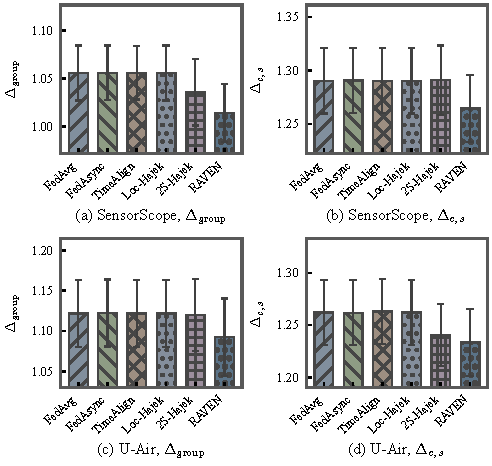
\includegraphics[width=\columnwidth]{fig3_e3_structural_mismatch.pdf}
\caption{Sealed same-backbone structural alignment on SensorScope and
U-Air (mean $\pm$ std over 20 paired seeds; lower is better).
(a)(b)~SensorScope $\Delta_{\mathrm{group}}$ and $\Delta_{c\text{-}s}$;
(c)(d)~U-Air $\Delta_{\mathrm{group}}$ and $\Delta_{c\text{-}s}$.
SensorScope RAVEN-MCS is support-conditional Design (Design on).  U-Air RAVEN-MCS in this
figure is full Design, not the support-conditional rows of
Table~\ref{tab:main_effectiveness}.}
\label{fig:e3_structural}
\end{figure}

\begin{figure}[t]
\centering
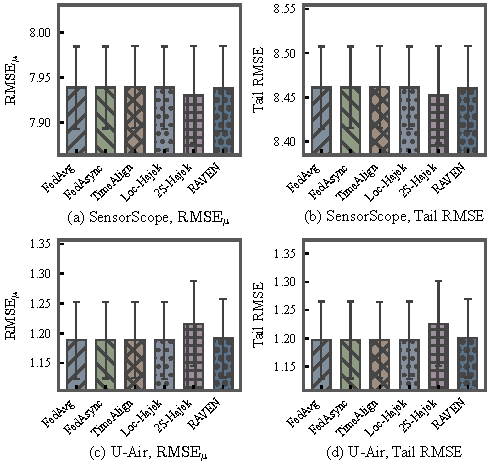
\includegraphics[width=\columnwidth]{fig4_e3_prediction_risk.pdf}
\caption{Sealed same-backbone deployment-target prediction risk
(mean $\pm$ std over 20 paired seeds; lower is better).
(a)(b)~SensorScope $\mathrm{RMSE}_{\mu}$ and Tail RMSE;
(c)(d)~U-Air $\mathrm{RMSE}_{\mu}$ and Tail RMSE.
U-Air RAVEN-MCS here is full Design.  The support-conditional U-Air row
($\mathrm{RMSE}_{\mu}=1.1131$) is in
Table~\ref{tab:main_effectiveness}.}
\label{fig:e3_prediction}
\end{figure}


\begin{figure}[t]
\raggedright
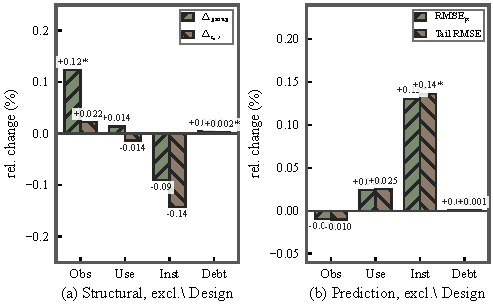
\includegraphics[width=\columnwidth]{fig6_e4_uair_excl_design.pdf}
\caption{U-Air component ablation excluding Design, magnified from
Fig.~\ref{fig:e4_ablation}.  (a)~Structural mismatch;
(b)~prediction risk.  Positive means removing the component worsens
the metric; $^\ast$ marks Holm-adjusted $p<0.05$.}
\label{fig:uair_excl_design}
\end{figure}

\subsection{Full E3 Method Context on the Comparable Datasets}
\label{app:e3_full_context}

\begin{table}[!htbp]
\centering
\caption{SensorScope full E3 method context (mean $\pm$ std over 20 seeds).
Lower is better.  $^\dagger$ denotes reference-only context.}
\label{tab:app_e3_sensorscope}
\scriptsize
\setlength{\tabcolsep}{3pt}
\begin{tabular*}{\columnwidth}{@{\extracolsep{\fill}}lccc}
\toprule
Method & $\mathrm{RMSE}_{\mu}$ & $\Delta_{\mathrm{group}}$ & $\Delta_{c\text{-}s}$\\
\midrule
Central-All$^{\dagger}$ & $7.6004\pm0.0695$ & -- & -- \\
Central-Delivered$^{\dagger}$ & $7.9291\pm0.0759$ & -- & -- \\
FedAvg-Window & $7.9389\pm0.0459$ & $1.0558\pm0.0288$ & $1.2903\pm0.0306$ \\
FedAsync-Window & $7.9391\pm0.0457$ & $1.0558\pm0.0287$ & $1.2906\pm0.0307$ \\
TimeAlign-Agg & $7.9395\pm0.0455$ & $1.0561\pm0.0282$ & $1.2904\pm0.0304$ \\
Local-Hajek & $7.9389\pm0.0459$ & $1.0558\pm0.0288$ & $1.2903\pm0.0306$ \\
TwoStage-Hajek & $7.9309\pm0.0543$ & $1.0353\pm0.0347$ & $1.2910\pm0.0324$ \\
Inst-Cal & $7.9380\pm0.0473$ & $1.0141\pm0.0305$ & $1.2644\pm0.0312$ \\
Debt-Cal & $7.9399\pm0.0463$ & $1.0272\pm0.0275$ & $1.2710\pm0.0298$ \\
RAVEN-MCS & $7.9380\pm0.0473$ & $1.0139\pm0.0305$ & $1.2644\pm0.0312$ \\
RAVEN-SimOracle$^{\dagger}$ & $7.9373\pm0.0455$ & $1.0160\pm0.0327$ & $1.2709\pm0.0301$ \\
\bottomrule
\end{tabular*}
\end{table}

\begin{table}[!htbp]
\centering
\caption{U-Air full E3 method context (mean $\pm$ std over 20 seeds).
Lower is better.  $^\dagger$ denotes reference-only context.
RAVEN-MCS in this table is full Design, not the support-conditional U-Air assignment.}
\label{tab:app_e3_uair}
\scriptsize
\setlength{\tabcolsep}{3pt}
\begin{tabular*}{\columnwidth}{@{\extracolsep{\fill}}lccc}
\toprule
Method & $\mathrm{RMSE}_{\mu}$ & $\Delta_{\mathrm{group}}$ & $\Delta_{c\text{-}s}$\\
\midrule
Central-All$^{\dagger}$ & $1.0556\pm0.0566$ & -- & -- \\
Central-Delivered$^{\dagger}$ & $1.1782\pm0.0981$ & -- & -- \\
FedAvg-Window & $1.1882\pm0.0649$ & $1.1218\pm0.0417$ & $1.2621\pm0.0309$ \\
FedAsync-Window & $1.1883\pm0.0648$ & $1.1223\pm0.0416$ & $1.2619\pm0.0310$ \\
TimeAlign-Agg & $1.1884\pm0.0642$ & $1.1218\pm0.0417$ & $1.2630\pm0.0310$ \\
Local-Hajek & $1.1882\pm0.0649$ & $1.1218\pm0.0417$ & $1.2621\pm0.0309$ \\
TwoStage-Hajek & $1.2160\pm0.0716$ & $1.1196\pm0.0445$ & $1.2406\pm0.0297$ \\
Inst-Cal & $1.1911\pm0.0659$ & $1.0924\pm0.0479$ & $1.2334\pm0.0320$ \\
Debt-Cal & $1.1893\pm0.0654$ & $1.0976\pm0.0457$ & $1.2400\pm0.0314$ \\
RAVEN-MCS & $1.1911\pm0.0659$ & $1.0924\pm0.0479$ & $1.2334\pm0.0320$ \\
RAVEN-SimOracle$^{\dagger}$ & $1.1914\pm0.0654$ & $1.0922\pm0.0483$ & $1.2342\pm0.0325$ \\
\bottomrule
\end{tabular*}
\end{table}

The central methods provide prediction-only reference context and therefore
have no distributed structural-mismatch entry.  RAVEN-SimOracle is a controlled
reference rather than a deployable baseline.  NSW-Traffic is intentionally not
added to this homogeneous E3 table because its reused cross-vintage path is not
scientifically comparable to the SensorScope/U-Air formal blocks.

\subsection{Four-Block Per-Group RMSE}
\label{app:block_rmse}

Table~\ref{tab:app_block_rmse} reports the four UTC-block scores whose
maximum is $\mathrm{WorstGroupRMSE}$ in
Table~\ref{tab:main_effectiveness}.  The blocks are the public
deployment groups $00$--$06$, $06$--$12$, $12$--$18$, and $18$--$24$~UTC.
This table does not introduce a new ranking rule.  On both datasets the
worst block is $g=2$ ($12$--$18$~UTC).  The pre-registered under-served
block $g^{\star}$ coincides with that worst block on SensorScope and
does not on U-Air.

\begin{table}[!t]
\centering
\caption{Four-block $\mathrm{RMSE}_g$ (mean $\pm$ std over 20 paired
seeds).  Lower is better.  $\mathrm{WorstGroupRMSE}=\max_g\mathrm{RMSE}_g$.
Support-conditional RAVEN is the E3 utility protocol.  U-Air full Design is a labeled
diagnostic row.  Source: G2 stored per-seed block scores.}
\label{tab:app_block_rmse}
\scriptsize
\setlength{\tabcolsep}{2.2pt}
\begin{tabular*}{\columnwidth}{@{\extracolsep{\fill}}llccccc}
\toprule
Dataset & Method & $g{=}0$ & $g{=}1$ & $g{=}2$ & $g{=}3$ & WG\\
\midrule
\multirow{5}{*}{SS}
& FedAvg-Window & $7.4912{\pm}0.0464$ & $7.5873{\pm}0.0444$ & $8.6716{\pm}0.0471$ & $8.2084{\pm}0.0460$ & $8.6716{\pm}0.0471$\\
& TwoStage-Hajek & $7.4831{\pm}0.0549$ & $7.5795{\pm}0.0523$ & $8.6633{\pm}0.0556$ & $8.2004{\pm}0.0549$ & $8.6633{\pm}0.0556$\\
& FedAU-Window & $7.4887{\pm}0.0512$ & $7.5848{\pm}0.0491$ & $8.6691{\pm}0.0522$ & $8.2059{\pm}0.0510$ & $8.6691{\pm}0.0522$\\
& ObsUse-Window & $7.4815{\pm}0.0517$ & $7.5780{\pm}0.0496$ & $8.6618{\pm}0.0528$ & $8.1988{\pm}0.0516$ & $8.6618{\pm}0.0528$\\
& RAVEN (SCD) & $7.4903{\pm}0.0479$ & $7.5864{\pm}0.0457$ & $8.6707{\pm}0.0486$ & $8.2075{\pm}0.0476$ & $8.6707{\pm}0.0486$\\
\midrule
\multirow{6}{*}{UA}
& FedAvg-Window & $1.1751{\pm}0.0579$ & $1.1922{\pm}0.0606$ & $1.2596{\pm}0.0709$ & $1.1521{\pm}0.0628$ & $1.2596{\pm}0.0709$\\
& TwoStage-Hajek & $1.2009{\pm}0.0623$ & $1.2194{\pm}0.0649$ & $1.2907{\pm}0.0753$ & $1.1800{\pm}0.0670$ & $1.2907{\pm}0.0753$\\
& FedAU-Window & $1.1023{\pm}0.0545$ & $1.1153{\pm}0.0576$ & $1.1701{\pm}0.0689$ & $1.0729{\pm}0.0598$ & $1.1701{\pm}0.0689$\\
& ObsUse-Window & $1.1016{\pm}0.0544$ & $1.1145{\pm}0.0576$ & $1.1692{\pm}0.0689$ & $1.0721{\pm}0.0598$ & $1.1692{\pm}0.0689$\\
& RAVEN (full) & $1.1779{\pm}0.0583$ & $1.1953{\pm}0.0611$ & $1.2630{\pm}0.0716$ & $1.1552{\pm}0.0633$ & $1.2630{\pm}0.0716$\\
& RAVEN (SCD) & $1.1025{\pm}0.0578$ & $1.1155{\pm}0.0611$ & $1.1703{\pm}0.0734$ & $1.0732{\pm}0.0636$ & $1.1703{\pm}0.0734$\\
\bottomrule
\end{tabular*}
\end{table}

\subsection{Runtime Diagnostic from Existing E2 Logs}
\label{app:runtime}

Table~\ref{tab:app_runtime} reports measured wall-clock runtime only as an
implementation diagnostic.  The ``all scenarios'' column aggregates six
E2 scenarios and 20 seeds (120 runs per method); the Complete-aligned column
contains 20 runs per method.  These measurements are not a scalability claim.

\begin{table}[!htbp]
\centering
\caption{Existing E2 runtime diagnostic in seconds (mean $\pm$ std).}
\label{tab:app_runtime}
\footnotesize
\setlength{\tabcolsep}{3.5pt}
\begin{tabular*}{\columnwidth}{@{\extracolsep{\fill}}lcc}
\toprule
Method & All scenarios & Complete-aligned\\
\midrule
FedAvg-Window & $71.426\pm5.105$ & $69.278\pm2.287$ \\
FedAsync-Window & $71.418\pm4.863$ & $70.186\pm3.531$ \\
TimeAlign-Agg & $71.244\pm5.225$ & $69.217\pm2.554$ \\
TwoStage-Hajek & $71.781\pm8.017$ & $69.829\pm3.670$ \\
RAVEN-MCS & $72.669\pm4.243$ & $71.070\pm1.292$ \\
\bottomrule
\end{tabular*}
\end{table}

Across these runtime rows (Table~\ref{tab:app_runtime}) there are no recorded
non-finite model parameters, non-finite losses, denominator-zero events, or
recorded P2 solver failures.  The diagnostic supports implementation sanity only and does not
establish asymptotic system efficiency.

\subsection{Provenance of the w/o-Design Endpoint Trade-off}
\label{app:design_provenance}

The Design ablation in Section~\ref{subsec:eval_rq3} exhibits an endpoint
trade-off on U-Air.  A paired-window provenance audit covers
774 windows.  Opportunity, observation, usable-update, and
registration hashes are identical between full RAVEN and w/o-Design throughout
the audited set.  Differences first arise from the positive design-weight/P2
support induced after the Design ratio is removed.  This confirms that the
ablation effect is a weight-support consequence of the intended intervention,
not selection-trace leakage.

\paragraph{Scope of the supplementary evidence.}
The appendices report only supplementary statistics and proofs needed to
interpret the main experiments.  They do not introduce an additional
evaluated dataset or a cross-vintage Traffic E3 comparison.



\end{document}
